\documentclass[10pt]{article}
\usepackage{mathtools}
\usepackage{amsmath}
\usepackage{fancybox}
\usepackage[margin=1.25in]{geometry}
\usepackage{tikz}
\usetikzlibrary{trees,shapes,snakes}
\newcommand{\tab}[1]{\hspace{.05\textwidth}\rlap{#1}}
\begin{document}
\vspace*{\fill}
\begin{Huge}
\begin{center}
HW2\\
Name: Ayush Jain\\
UNI: aj2672
\end{center}
\end{Huge}
\vspace*{\fill}
\newpage
\section{Problem 1}
\textbf{Exercise 6.5-9}\\
A: 2-D array storing k arrays of n elements each\\
B: Stores the current min-heap of elements\\
C: Stores the mapping of the element to the list it belongs to.\\
D: Stores the mapping of the element to its index in A.\\
r: index in result string\\\\
Note: The Build-Mean-Heap and Min-Heapify refer to the standard algorithms from CLRS and lectures modified to keep information of the index j in the list i to which an element in the heap B belongs to. For the element B[i], C[i] gives the sorted list and D[i] gives the index in that list to which the element belongs. Since, the changes to store this information is a part of our main loop, it wont affect the time complexity of the original algorithm.\\
Merge(A, k, n)
\begin{enumerate}
\item for (i = 1 upto k)
\item\tab{B[i] = A[i][1];}
\item\tab{C[i] = i;}
\item\tab{D[i] = 1;}
\item Build-Min-Heap(B, C, D, k);
\item while (B is not empty)
\item	\tab{result[r++] = B[1]; //The first element of B will always be the minimum.}
\item	\tab{if(D[1] $<$ n)}
\item	\tab{\tab{D[1]++;}}
\item \tab{\tab{key = A[C[1]][D[1]];}}
\item	\tab{\tab{Heap-Replace-Root(B, key, C, D);}}
\end{enumerate}
Heap-Replace-Key(B, key, C, D)
\begin{enumerate}
\item B[1] = key;
\item Min-Heapify(B, 0, C, D)
\end{enumerate}
The above algorithm, first extracts the first elements of all the k sorted lists and save them to array B. Then, we heapify this array to transform it into a heap. From, this operation we get the minimum of all the elements of the entire result set. Then we run a loop to save this minimum element into our result set, replace it with the next element of the array it belongs to and run a Min-heapify operation to again get the next smallest element of our result set.\\
For the algorithm, the time complexity computation is as follows:
Steps 1 to 4 take have complexity O(k)\\
Step 5 has a complexity of O(k)\\ (Building a heap takes O(k) time. From CLRS)
Step 11 has a complexity of O(log k) and it occurs n times inside the while loop. Hence, it is safe to say that Step 6 to 11 has a complexity of O(n log k)\\
Hence, complexity of the entire operation = O(n logk) + 2*O(k) = O(nlogk).\\\\
Loop Invariant Proof:\\
\textbf{Initialization:} Prior to the first iteration of the loop between rows 6 and 11, we extract the smallest element of each sorted list and build a min heap out of those elements. So, the minimum out of the set of these k elements which is also the minimum of all n elements of all k lists taken together is at the root of this heap. This is the first element of our result set.\\
\textbf{Maintenance:} To see that each iteration maintains the loop invariant, we can assume that we have the i smallest elements of our result set. At the beginning of the $i+1^{th}$ iteration, we have the $(i+1)^th$ minimum at the root of our min-heap. We store it in our result set. Now we call the Heap-Replace-Key to replace it with the next element of its original list. And then, we call the heapify algorithm. This will reduce our modified array B to a min-heap. So, the minimum of all the elements in B will be at the root after this iteration. This will also be the $(i+2)^{th}$ element of our result set.\\
\textbf{Termination:} At termination, we have an empty B, which means that all our sorted lists have been consumed by the algorithm. This also means that the result set has data from all k sorted lists in a sorted order.
\newpage
\section{Problem 2}
\textbf{Problem 6-3}\\
a. One 4x4 Young Tablaus matrix from the given data would look like:
\[
	\begin{bmatrix}
		2 & 3 & 4 & \infty\\
		5 & 8 & 9 & \infty\\
		12 & 14 & 16 & \infty\\
		\infty & \infty & \infty & \infty
	\end{bmatrix}		
\]\\\\\\
b. The entries of a Young Tablaus matrix in each row are in sorted order from left to right and the entries of each column are in sorted order from top to bottom. So, if $Y[1,1] = \infty$, then all the elements in the first row and first column are equal to $\infty$. So, this means Y[2,1] is also $\infty$, which in turn means that all elements of second row are also $\infty$. Extending the same logic to the entire matrix, we an say that all the elements of the matrix are $\infty$. Since we treat $\infty$ elements as non existent, our matrix is essentially empty.\\\\
if Y[m,n], i.e the last element of our matrix $ < \infty$, it means that all the elements in the $m^{th}$ row $and n^{th}$ column are $< \infty$. The above set includes, Y[m-1, n] and Y[m, n-1]. This implies that all the elements in $(m-1)^{th}$ row and $(n-1)^{th}$ column are also $< \infty$. Extending this logic to the entire matrix, we get that all the elements of the matrix are $< \infty$. Hence, we can say that the matrix is full.\\\\\\
c. All rows and columns in a Young Tableaux matrix are sorted. Hence, the first element, i.e., Y[1,1] will always be the smallest element of such a matrix\\\\
A: input Young Tableaus matrix\\
m: number of rows in A\\
n: number of columns in A\\\\
EXTRACT-MIN(A, m, n)
\begin{enumerate}
\item min = A[1,1]
\item A[1,1] = A[m, n]
\item $A[m, n] = \infty$
\item Young-Tableaus-Reduction(A, 1, 1, m, n)
\item return min\\
\end{enumerate}
Young-Tableaus-Reduction(A, i, j, m, n)
\begin{enumerate}
\item minRow = i;
\item minCol = j;
\item if ((i+1 $<$ m) \&\& $(A[i][j] > A[i+1][j]$)
\item \tab{minRow = i+1;}
\item \tab{minCol = j;}
\item if ((j+1 $<$ n) \&\& $(A[minRow][minCol] > A[i][j+1]$)
\item \tab{minRow = i;}
\item \tab{minCol = j+1;}
\item if $(minRow \neq i) \| (minCol \neq j)$
\item \tab{swap A[i][j] with A[minRow][minCol]}
\item \tab{Young-Tableaus-Reduction(A, minRow, minCol, m, n)}\\
\end{enumerate}
In the above algorithm, we extract out the first element of the matrix, since that is the smallest element. We replace it with the last element and set the last element $= \infty$. Then, we go over the entire matrix recursively. We compare each element with the one directly below and with the one directly on the right. The minimum of the two is selected and swapped with the original element. The breaking condition is when the element on the right and the element below are greater. \\\\
Loop Invariant Proof:\\
\textbf{Initialization:} As discussed above, the minimum element is always the first element, or A[1][1]. We extract out this element from the matrix and replace it with A[m][n], the last element of the matrix. We put $\infty$ at the position of this last element. Prior to the first iteration of the loop, the elements before $i<1$ and $j<1$ are in the Young Tableaus form.\\
\textbf{Maintenance:} After $i^{th}$ iteration, lets say we are at $l^{th}$ row and $m^{th}$ column. This means all elements $a_{p,q}$ for $p<l$ and $q<m$ follow the Young Tableaus form. Now we compare $a_{l,m}$ with $a_{l+1,m}$ and $a_{l,m+1}$ and swap it with the minimum of the two. Lets say that $a_{l+1,m}$ was the minimum. Hence, now we are at $(l+1)^{th}$ row and $m^{th}$ column and all elements $a_{p,q}$ for $p<l+1$ and $q<m$ are in the Young Tableaus form.\\
\textbf{Termination:} The ending condition occurs when our element $a_{p,q}$ is less than both $a_{p+1,q}$ and $a_{p,q+1}$. This means that the element follows in its current position the Young Tableaus nature of the matrix. Since, all the elements except for the first were already in the desired form, we just had to find the correct position for the first element, which has been reached.\\\\
Time Complexity Proof:\\
After each recursion, we move down one row or move by one column towards right. That is, with every recursion our problem set reduces by 1. We can write the recurrence tree by:\\
T(m+n) = T(m+n-1) + 1\\
Replacing, m+n = p\\
T(p) = T(p-1) + 1\\
Number of levels are given by :\\
p-h = 1\\
h = p-1\\
Hence, T(p) = 1+1+1+ .... p-1 terms\\
T(p) = O(p)= O(m+n)\\

The recurrence tree of the above relation is given by: \\
\ovalbox{
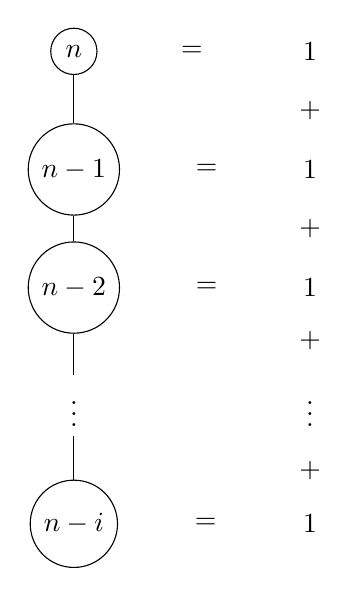
\begin{tikzpicture}[level/.style={sibling distance=0mm/#1}]
\node [circle,draw] (z){$n$}
  child {node [circle,draw] (a) {$n-1$}
    child {node [circle,draw] (b) {$n-2$}
      child {node {$\vdots$}
        child {node [circle,draw] (d) {$n-i$}}
      } 
    }
  }
    child [grow=right] {node (q) {$=$} edge from parent[draw=none]
          child [grow=right] {node (q) {$1$} edge from parent[draw=none]
            child [grow=down] {node (r) {$1$} edge from parent[draw=none]
              child [grow=down] {node (s) {$1$} edge from parent[draw=none]
                child [grow=down] {node (t) {$\vdots$} edge from parent[draw=none]
                  child [grow=down] {node (u) {$1$} edge from parent[draw=none]}
                }
              }
            }
          }
        };
\path (q) -- (r) node [midway] {+};
\path (s) -- (r) node [midway] {+};
\path (s) -- (t) node [midway] {+};
\path (a) -- (r) node [midway] {=};
\path (t) -- (u) node [midway] {+};
\path (b) -- (s) node [midway] {=};
\path (d) -- (u) node [midway] {=};
\end{tikzpicture}}\\\\\\\\
d. Insert-Element(A, key)
\begin{enumerate}
\item A[m, n] = key
\item Young-Tableaus-Reduction(A, i, j)
\item return min\\
\end{enumerate}
Young-Tableaus-Reduction(A, i, j)
\begin{enumerate}
\item maxRow = i;
\item maxCol = j;
\item if ((i-1 $>$ 0) \&\& $(A[i][j] < A[i-1][j]$)
\item \tab{maxRow = i-1;}
\item \tab{maxCol = j;}
\item if ((j-1 $>$ n) \&\& $(A[maxRow][maxCol] < A[i][j-1]$)
\item \tab{maxRow = i;}
\item \tab{maxCol = j-1;}
\item if $(maxRow \neq i) \| (maxCol \neq j)$
\item \tab{swap A[i][j] with A[maxRow][maxCol]}
\item \tab{Young-Tableaus-Reduction(A, maxRow, maxCol, m, n)}\\
\end{enumerate}
For insertion we follow the exact opposite of the algorithm outlined for the above extract minimum problem. Since the question says a non full matrix, we know that the last element is $\infty$. To insert we can add the new element at Y[m,n]. Then recursively we find the max(Y[i-1,j], Y[i,j-1]) and swap it with Y[i,j]. If Y[i,j] is in fact the minimum element then we have already reached the correct position of the key and the program ends.\\\\
Similar to above, the time complexity of the problem is O(m+n). This is because the worst case would be if the new key is the smallest element of the matrix and we traverse the entire matrix from Y[m,n] to Y[1,1]. After each iteration, the problem reduces from a size of i+j to i+j-1 (either we travel one position upwards or towards left). So we get a recurrence tree similar to the above problem and also the same complexity, i.e., O(m+n).\\\\
Loop Invariant Proof:\\
\textbf{Initialization:} As discussed above, since the matrix is non-full, the last element or A[m][n] is always non existential. We replace this element with our new key. Prior to the first iteration of the loop, the elements after $i>m$ and $j>n$ are in the Young Tableaus form.\\
\textbf{Maintenance:} After $i^{th}$ iteration, lets say we are at $l^{th}$ row and $m^{th}$ column. This means all elements $a_{p,q}$ for $p>l$ and $q>m$ follow the young tableaus form. Now we compare $a_{l,m}$ with $a_{l-1,m}$ and $a_{l,m-1}$ and swap it with the maximum of the two. Lets say that $a_{l-1,m}$ was the maximum. Hence, now we are at $(l-1)^{th}$ row and $m^{th}$ column and all elements $a_{p,q}$ for $p>l-1$ and $q>m$ are in the young tableaus form.\\
\textbf{Termination:} The ending condition occurs when our element $a_{p,q}$ is greater than both $a_{p-1,q}$ and $a_{p,q-1}$. This means that the element follows, in its current position the Young Tableaus nature of matrices.\\\\\\
e. As we showed above, inserting a number in a Young Tableaus takes O(m+n) = O(2n) time. Similarly, extracting the minimum out of a Young Tableaus matrix also takes O(m+n) = O(2n) time. If we take the array and insert all its elements into an empty Young Tableaus matrix repeatedly and then extract out of it the minimum elements one by one, that will give us a sorted array\\
\textbf{Algorithm:}\\
A:Array of $n^2$ numbers\\ 
B:Empty Matrix of nxn numbers\\
C:Sorted array A
\begin{enumerate}
\item Sort(A, n)
\item for i=1 till $n^2$
\item \tab{Insert-Element(B, A[i])}
\item for i=1 till $n^2$
\item \tab{C[i] = EXTRACT-MIN(B, n, n)}
\item return C
\end{enumerate}
The Step 2 and Step 4 both have complexity of O(2n) but they each run for $n^{2}$ time.\\
Complexity = $n^2O(2n)+n^2O(2n) = O(4n^3) = O(n^3)$\\\\\\\\\\\\
f. The following algorithm gives a way to find out, if a number is stored in a Young Tableaus matrix.\\
\textbf{Algorithm:}\\
A: Young Tableaus matrix of size mxn\\
key: the number to search for\\\\
Find-Key(A, m, n, key)
\begin{enumerate}
\item i=m, j=1
\item while($i \geq 1)$ \&\& $(j \leq n)$
\item \{
\item \tab{if (A[i][j] == key)}
\item \tab{\tab{return true\tab{\tab{//found, return}}}}
\item \tab{if (A[i][j] $>$ key)}
\item \tab{\tab{$i--$ \tab{\tab{//move upwards in the table}}}}
\item \tab{if (A[i][j] $<$ key)}
\item \tab{\tab{$j++$ \tab{\tab{//move towards right in the table}}}}
\item \}
\item return false
\end{enumerate}
\textbf{Explanation:}We start from the left bottom corner of the matrix, i.e., i=m and j=1. We compare our key with the element A[i][j]. If the key is greater, it means it is on the right to our element since the elements are sorted in a row. One the other hand if the key is smaller, it means we need to move up the matrix, since the elements in a column are sorted as well. We could have also started from the top right corner and moved our way towards the left bottom corner as well to achieve our result.\\\\
\textbf{Time Complexity: } In the worst case we go from bottom left corner to the upper right corner of the matrix. That is we make m+n steps. All the steps take O(1) time and are repeated m+n times(i from m to 1 and j from 1 to n, in the worst case).\\ Hence our time complexity: = O(m+n)\\\\
\textbf{Loop Invariant Proof:}\\
\textbf{Initiation:}Before the loop initializes, the key is not found. We our at the A[m][1] element. The key is not present on the left our starting element but may be present anywhere among the right holds true.\\
\textbf{Maintenance:} After the completion of the $k^{th}$ loop, lets say we are at the A[p][q] element. We compare the A[p][q] with our key. If both are equal, we return since we have validated the presence of our key. If the key is greater we move right towards A[p][q+1]. We have ruled out column($q^{th}$) from our possibilities, since we know that all its elements above p are smaller and below p are greater than our key. Otherwise, if the key is smaller we move up towards A[p-1][q]. We have ruled out $p^{th}$ row since all its elements to right are greater and to the left are smaller.\\
\textbf{Termination:}The loop finishes when:\\
a. We find our key in the matrix.\\
b. We have reached the extreme top right corner. We have validated the entire matrix and our key is not present in the matrix.\\
\newpage
\section{Problem 3}
\textbf{Problem 8.6}\\
a. For a given set of numbers, there is only one way to sort it. So, our problem is just to split the given array into two arrays of n elements each. Selecting n elements out of 2n elements can be done in $2n\choose n$ ways.\\\\\\
b. Lets assume we have two input arrays: \\
A: $a_{1}, a_{2}$\\
B: $a_{3}, a_{4}$\\
Below is the decision tree for such an input. The minimum number of comparisons in the best case are 2, when all the elements of first array are smaller than all of second. In the worst case 3 comparisons have to made when the loop runs till the last elements of each. 
Similarly, if we had n=3, the best and worst cases are 3 and 5 respectvely.\\
So, if we see our tree splits into two child at every node and every path gives us a an arrangement of the merged array depending on what my split was. For example if my sorted array is 1,2,3,4, the first leaf gives us the result when two arrays are: $\{a_1,a_2\}$ = \{1,3\} and $\{a_3,a_4\}$ = \{2,4\}.\\
\begin{figure}[ht!]
\centering
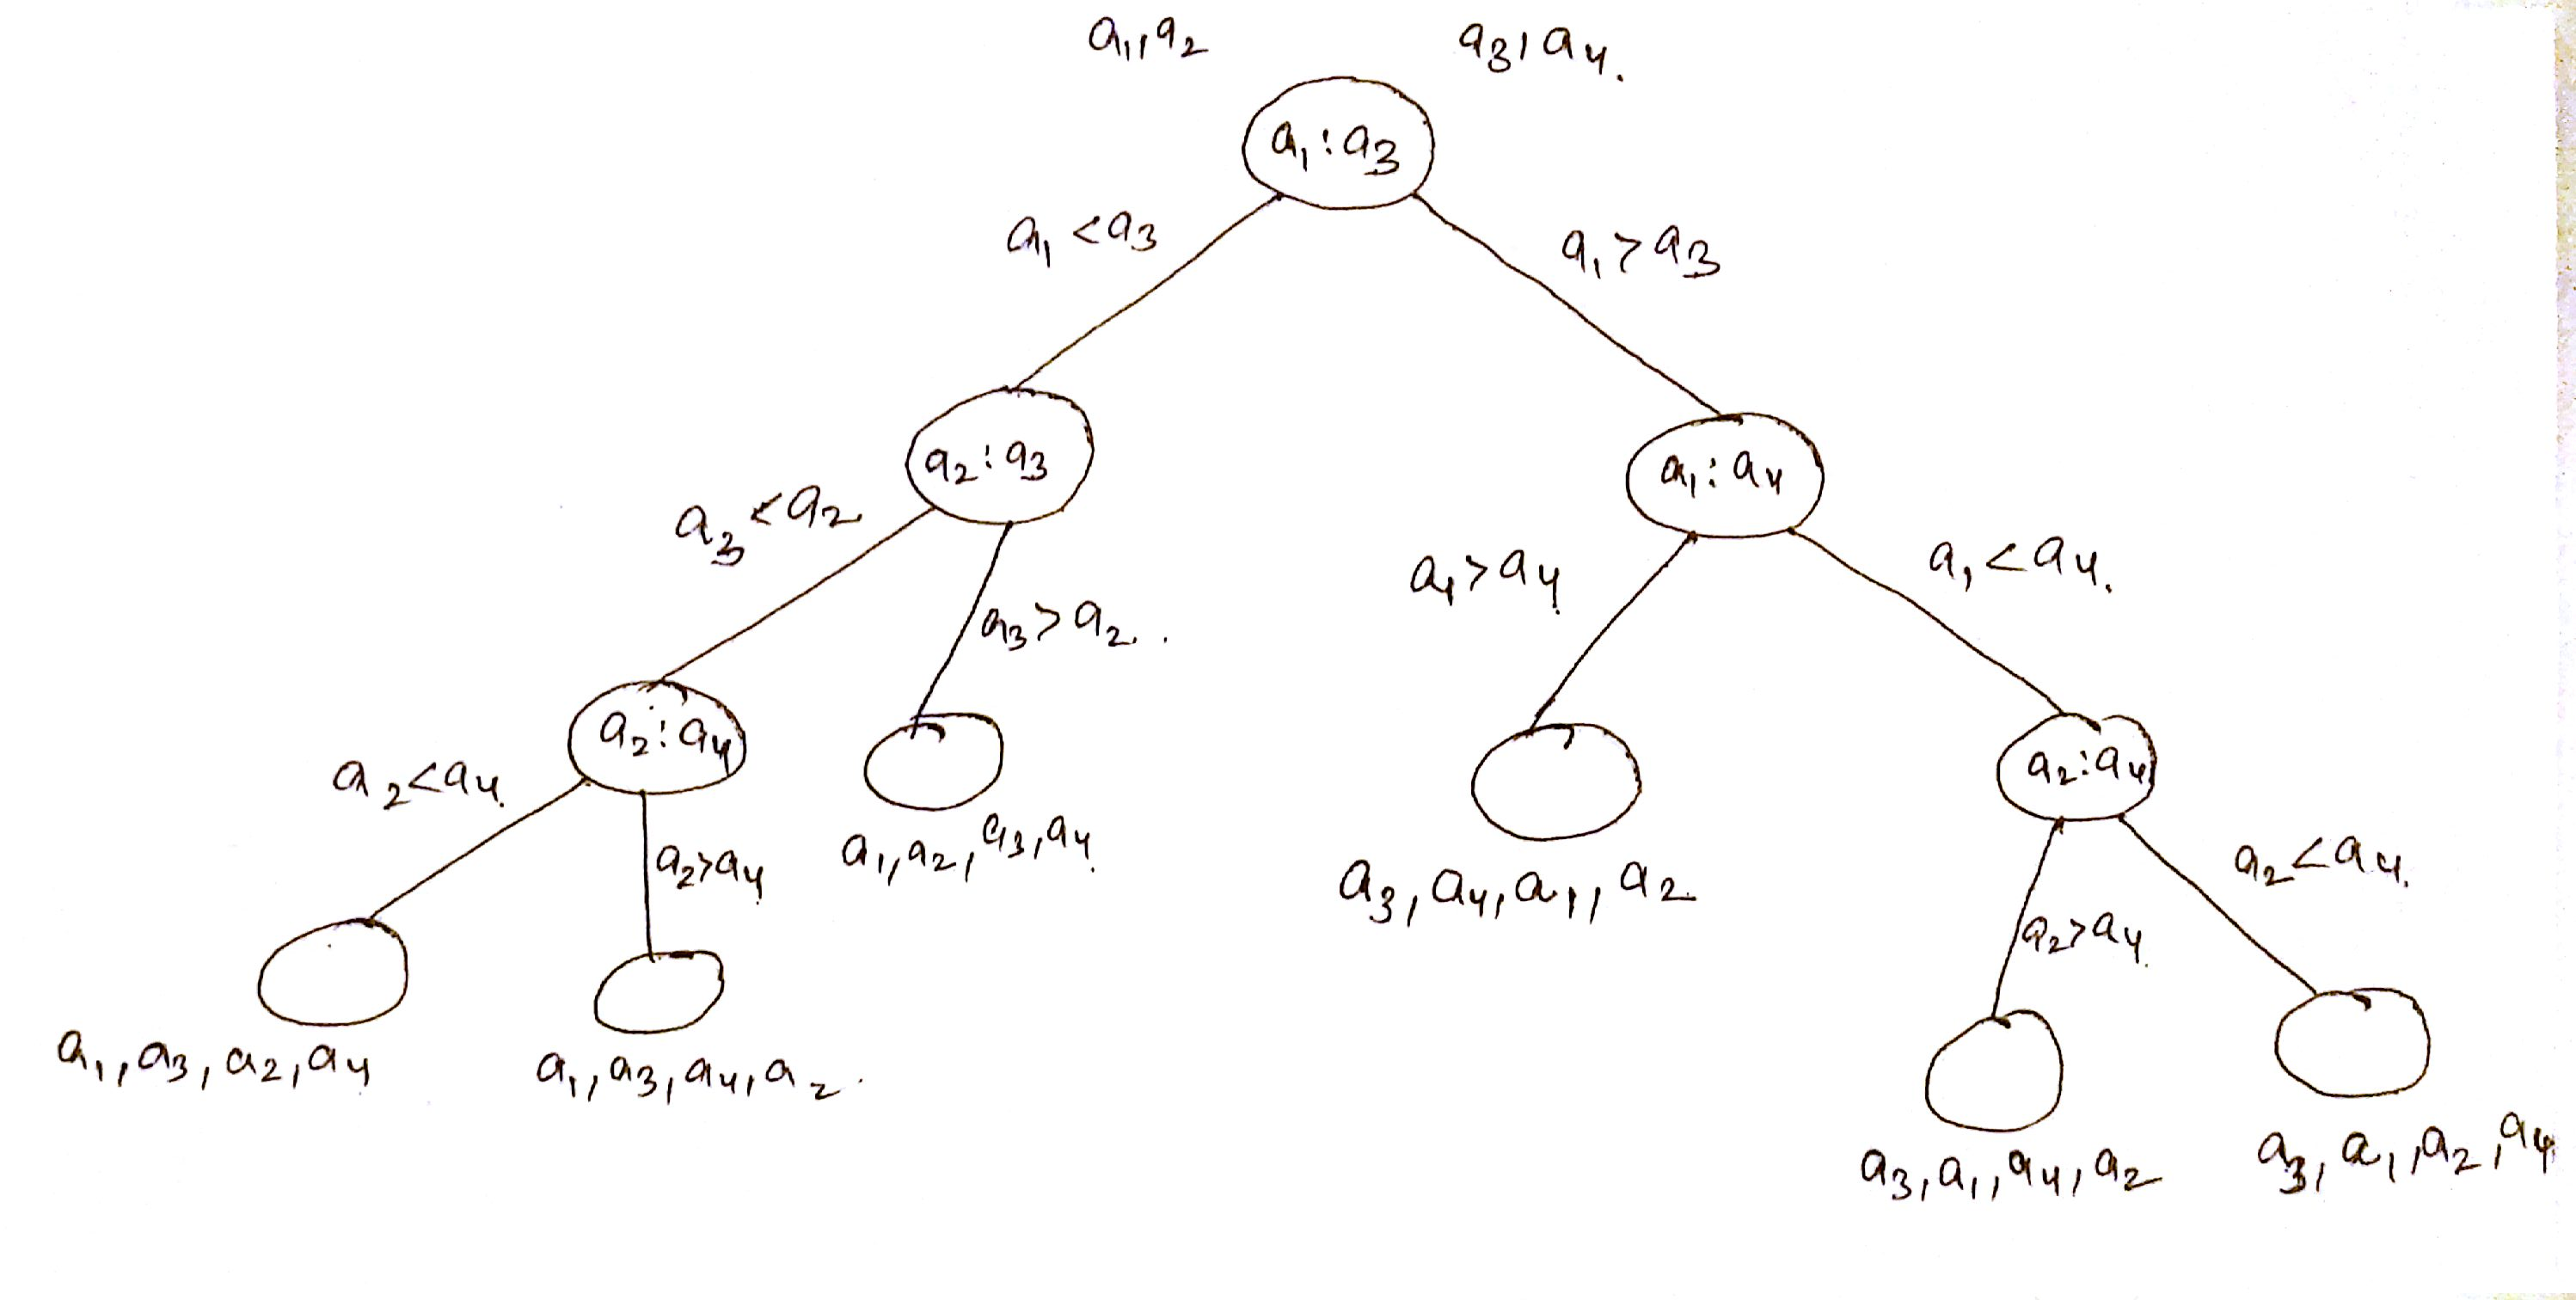
\includegraphics[width=120mm]{decisionTree.jpg}
\end{figure}\\
Since this is a binary tree, with leaves as its sorted array derived from different split of our 2n elements, we should have $2n\choose n$ leaf nodes. This means the height should be at least $\log {2n\choose n}$ and the height in this case represents the order of comparisons.\\
Now from polynomial expansion, we know that ${2n\choose n}$ always has the biggest value. It is greater than or equal to all ${2n\choose i}$ for i = 1,2,3 ..... 2n. So we can sum over all i and write it as:\\\\
$\sum_{i=0}^{2n}{2n\choose n} \geq \sum_{i=0}^{2n}{2n\choose i}$\\\\
$(2n+1){2n\choose n} \geq \sum_{i=0}^{2n}{2n\choose i}1^i1^{2n-1}$\\\\
The right side becomes: 
Using Binomial Expansion, the right side becomes: \\\\
 $(2n+1){2n\choose n} \geq (1+1)^{2n} = 2^{2n}$\\\\
Taking log on both sides: \\
$\log {2n\choose n} + \log ({2n+1}) \geq 2n$\\
\begin{equation}
\log {2n\choose n} \geq 2n - \log ({2n+1})
\end{equation}
Now for all values of c we can find n such that: $\log ({2n+1}) \leq cn$ \\
In other words: $\log ({2n+1}) = o(n)$ \\
Substituting in (1) we get:\\
\boxed{\log {2n\choose n} = 2n - o(n)}\\\\\\
c. Lets suppose that $\{a_1, a_2, a_3, .... a_n\}$ and $\{b_1, b_2, b_3, .... b_n\}$ be the two sorted arrays. Let suppose that in the sorted result we have $a_i$ and $b_j$ as two consecutive elements in the same order. We will assume that these were not compared. This can happen only when $a_i$ was compared to an element c and was found lower. As a result, we took $a_i$ and inserted it into our result  set. Then we extracted $b_j$ and compared it to c, found it lower and inserted it into the result set as well. But since the new element is always extracted from the same array as the previous one, it would mean that $a_i$ and $b_j$ belong to the same array. This contradicts our assumption. Hence, the elements have to be compared if they belong to different arrays.\\\\\\
d. In the result set, we have 2n elements. Using the above concept if we pair any two consecutive elements we get 2n-1 such pairs. The worst case occurs when any two consecutive elements belong to different lists and each pair correspond to one comparison. Hence, 2n-1 pairs leads to 2n-1 such comparisons.
\newpage
\section{Problem 4}
Exercise 9.3-6\\
The k-1 order statistics that divide a set into k quantiles would be given by $\dfrac{n}{k}, \dfrac{2n}{k}, \dfrac{3n}{k}, ... \dfrac{(k-1)n}{k}$.
Now if we split our array into two halves at each level for $\log k$ levels, we get k sets of $\dfrac{n}{2^{\log k}} = \dfrac{n}{k}$ elements. Thus we get our (k-1) order quantiles which will be the respective last elements of our k sets. \\
However, it will be this simple only when $\log k$ is an integer. Only in that case, our quantiles will be the last elements of the divided sets. If $\log k$ is not an integer, we still follow the same steps. At the end, however, instead of picking up the last elements of our k sets, we will have to find the n/k, 2n/k, ... (k-1)n/k elements through selection in our divided sets. This will need (k-1) selections in $\dfrac{n}{2^{\lfloor{\log k}\rfloor}}$ sets.\\\\
\textbf{Time Complexity:} The complexity is derived as:\\\\
$O(n\lfloor\log k\rfloor) + O((k-1)\dfrac{n}{2^{\lfloor{\log k}\rfloor}}) = O(n\log k) + O(n) = O(n\log k)$\\\\
\textbf{Algorithm:}\\
A: input array of size n\\
Quantiles(A, n)
\begin{enumerate}
\item for (int i=1; $i \leq \log k$; i++)
\item \tab{startIndex = 1}
\item \tab{endIndex = $n/2^{i-1}$}
\item \tab{for(int j=1; j $\leq 2^{i-1}$; j++)}
\item \tab{\tab{SELECT(A, startIndex, endIndex, (startIndex+endIndex)/2)}}
\item \tab{\tab{startIndex += $n/2^{i-1}$}}
\item \tab{\tab{endIndex += $n/2^{i-1}$}}
\item j = 1
\item for(int i = 1; $i<k$; i++)
\item \tab{if($j \ast \dfrac{n}{2^{\lfloor\log k\rfloor}} < i \ast n/k$}
\item \tab{\tab{j++}}
\item \tab{SELECT(partitions[j], 1, n/k, $i \ast n/k$)}
\end{enumerate}
\textbf{Explanation:} The above algorithm first splits the input array into halves repeatedly upto $\log k$ levels. These sets are stored in the partitions array, with each row one such partition. For example, the partition[1] is the first partition, partition[2] the second and so on. Then in the steps from 9 to 12, we perform (k-1) selections of $i \ast n/k$ indexes where i = 1,2,3, ... (k-1). We check if the $i \ast n/k$ is greater than the last index stored in the current partition, we increment the counter to the next partition.\\\\\\\\
Exercise 9.3-8\\\\
A, B: input arrays\\
a, b: index range of A\\
c, d: index range of B\\\\
\textbf{Algorithm:}\\
MEDIAN(A, B, a, b, c, d)
\begin{enumerate}
\item if $(((b-a+1) \leq 2)\|((d-c+1)/2))$
\item \tab{C = A[a:b]U B[c:d]}
\item \tab{if C.length \% 2 == 0)}
\item \tab{\tab{return C[C.length/2]}}
\item \tab{else}
\item{\tab{\tab{return C[(C.length + 1)/2]}}}
\item if (A[(a+b)/2] == B[(c+d)/2])
\item \tab{return A[(a+b)/2]}
\item if(A[(a+b)/2] $>$ B[(c+d)/2])
\item \tab{return MEDIAN(A, B, a, (a+b)/2, (c+d)/2, d)}
\item if(A[(a+b)/2] $<$ B[(c+d)/2])
\item \tab{return MEDIAN(A, B, (a+b)/2, b, c, (c+d)/2)}
\end{enumerate}
\textbf{Explanation:} Since both of our arrays are sorted, we can compare the medians of the arrays in a single operation. Lets say that A[p] and B[q] represent the medians of A and B respectively. Lets assume that A[p] $>$ B[q]. Then the elements greater than A[p] are certainly greater than the median of the collective set. This is because we know that the first n/2 elements of each array are smaller than A[p] and hence we have at least the first n elements out of the total 2n elements. We know that the $n^{th}$ element of the sorted 2n elements is our median. So we can discard the elements in A, with indexes greater than p. Similarly, the elements of B smaller than q can also be discarded. Hence, our problem size reduces from 2n to n in O(1) time. Now we perform this iteration repeatedly on the remaining elements of A and B, till either we find the median or we reach a stage where the number of elements in at least one of the arrays are reduced to 2. Once the number of elements in any one of the array reduces to 2, we calculate the median by combining the elements, sorting them and picking the $\lceil n/2 \rceil^{th}$ element.\\\\
\textbf{Time Complexity: } As discussed above the time complexity of the function is given by:\\
T(n) = T(n/2) + 1\\
T(n) = T(n/4) + 1 + 1\\
T(n) = 1 + 1 + 1 .... $\log n$ times\\
T(n) = O($\log n$)\\\\
In the end, the selection of the median adds some complexity but it is independent of n. Since the total number of elements for which we want to find the median is 4 or 5, the complexity added is O(4) or O(5) and this can be ignored with $O(\log n)$.
\newpage
\section{Problem 5}
\setcounter{equation}{0}
Problem 9.2\\
a. Unsorted array, A: $x_1, x_2, x_3, .... x_n$\\
Lets say that the sorted array is given by:\\
B: $z_1, z_2, z_3, .... z_n$\\
Then, the median is given by: $z_k$,
where, $k=\dfrac{n}{2}$ for even n and $k = \dfrac{n+1}{2}$ for odd n\\
Now for these k, 
\[
  \sum_{i=0}^{k-1} w_i = 
  \begin{cases} 
      \dfrac{1}{2} - \dfrac{1}{n}    \hfill & \text{ if $n$ is even} \\\\
      \dfrac{1}{2} - \dfrac{1}{2n} \hfill & \text{ if $n$ is odd} \\
  \end{cases}
\] 
and 
\[
  \sum_{i=k+1}^{n} w_i = 
  \begin{cases} 
      \dfrac{1}{2}    \hfill & \text{ if $n$ is even} \\\\
      \dfrac{1}{2} - \dfrac{1}{2n} \hfill & \text{ if $n$ is odd} \\
  \end{cases}
\] 
Which fits our definition of a weighted median. k is the maximum term below which the sum of terms is less than half. If we add $z_k$, the sum for both goes above 1/2. Also, the sum of all terms greater than $z_k$ is also less than or equal to 1/2 for both odd and even n. Hence, $z_k$ is our median.\\\\\\
b. A: input array of size n\\
Weighted-Median(A, n)
\begin{enumerate}
\item B = MergeSort(A, n)
\item sum = 0
\item for(i=1 to n)
\item \tab{sum += weight of B[i]}
\item \tab{if $(sum \geq 1/2)$}
\item \tab{\tab{return B[i]}}
\end{enumerate}
\textbf{Explanation:} First we sort our array in increasing order using merge sort. After that we iterate over the sorted array and find out the sum of the weights of its element. As soon as the sum becomes greater than or equal to 1/2, we break out of the loop. We know that the current element is our weighted median as its the greatest element below which the sum of all elements is less than 1/2.\\\\
\textbf{Time Complexity:} Following is the time complexity of individual steps:
\begin{enumerate}
\item O($n\log n$)
\item O(1)
\item Steps 4 to 6 O(1) repeated n times.
\end{enumerate}
Hence the total complexity: O($n \log n$) + O(1) + O(n) = $O(n\log n)$\\\\\\
c. Lets assume A:$x_1, x_2, x_3, .... x_n$ is our input array.\\
To find the weighted median, we follow the steps of SELECT algorithm till finding the pivot, k. However, during partitioning, we find the sum of elements of on both side of our pivot. If the sum of elements with indexes $i < k$ and sum of elements $i > k$ satisfy our weighted median condition, then $x_k $ is our weighted median. If the sum of elements with indexes $i<k$ is greater than 1/2, we recurse on the left hand side set and find our weighted median. If the sum of elements with indexes $i>k$ is greater than 1/2, then we calculate the sum of elements on the left, lets say w. Then we recurse on the right set of the pivot and consider the weighted median condition equal to 1/2-w instead of 1/2.\\
The time complexity is the same as that of SELECT. While iterating over the elements, instead of calculating the number of elements on both side of the pivot we calculate the sum of weights of elements on both sides. Both are O(1) operations and hence the time complexity does not change.\\\\\\
d. We have to minimize the sum: 
\begin{equation}
\sum_{i=1}^{n}w_{i}d(p,p_i) = \sum_{i=1}^{n}w_{i}|p-p_i|
\end{equation}
Lets assume a sorted array of points: $p_1, p_2, p_3, p_4, p_5$. Then the median is obviously $p_3$. Lets assume the weights, $w_1, w_2, w_3, w_4, w_5$ in such a way that the weighted median is also $x_3$.\\
Lets try to find the sum when p = $p_4$.\\\\
$\sum_{i=1}^{n}w_{i}|p-p_i| = w_1(p_4 - p_1) + w_2(p_4-p_2) + w_3(p_4-p_3) + w_5(p_5 - p_4))\\\\
= w_1(p_3-p_1) + w_2(p_3 - p_2) + w_4(p_4 - p_3) + w_5(p_5-p_3) + (p_4-p_3)(w_1 + w_2 + w_3 - w_4 - w_5)\\\\
= \sum_{i=1}^{n}wd|p_3, p_i| + (p_4-p_3)(w_1 + w_2 + w_3 - w_4 - w_5)$\\\\
Keeping in mind that $p_3$ is our weighted median, the second term on the right is always positive. This is because the value $(w_4 + w_5)$ is always less than or equal to 1/2 and the value $(w_1 + w_2 + w_3)$ is always greater than or equal to half. Hence, it is easy to see that the value for p=$p_4$ is greater than that for the weighted median. If we try for other $p_{i}'s$ or for greater number of inputs as well, then also we get the same result. Hence, it is safe to say that the minima is always achieved for weighted median.\\
\\\\\\
e. For a two dimensional system, every point p is represented as (x,y). Hence the sum becomes: \\\\
$\sum_{i=1}^{n}w_{i}d(p,p_i) = \sum_{i=1}^{n}w_{i}(|x - x_i| + |y - y_i|)\\\\
= \sum_{i=1}^{n}w_{i}|x - x_i| + \sum_{i=1}^{n}w_{i}|y - y_i|)$\\\\
Hence, this can be treated as two distinct problems for x and y taken separately. Using the result proved in (d) above, we can find the minimum value of x and y separately and then combine them together to derive our result.
\newpage
\section{Problem 6}
Exercise 5.3-2\\
Lets assume we have an array $x_1, x_2, x_3$. Now according to the algorithm, on each iteration i we select an element $x_i$ and swap it with a random element chosen from $x_{i+2}, x_{i+3}, .. x_{i+n}$. One possible combination of these elements can be $x_3, x_2, x_1$. Since this is not an identity combination, this result should be achievable using the above algorithm. Lets try to follow the algorithm step by step and try to achieve this result:\\\\
\textbf{Initial state}: $x_1, x_2, x_3$\\
\textbf{1st iteration}: $x_1$ needs to be replaced by $x_3$, since the final result has $x_3$ as the first element.\\
Hence, after first iteration : $x_3, x_2, x_1$.\\
\textbf{2nd iteration: } $x_2$ needs to be swapped with 3rd element, since that is the only choice. Hence, after second iteration: $x_3, x_1, x_2$.\\\\
Hence, as we saw it is impossible to form the list $x_3, x_2, x_1$ from $x_1, x_2, x_3$ using the above algorithm. Rather, the only two outputs from our array using the above algorithm can be: $x_3, x_1, x_2$ or $x_2, x_3, x_1$ depending on the element we chose to swap $x_1$ with in our first iteration. The possible number of combinations however should be 5, if we leave the identity combination. Hence, the above algorithm is not random.\\\\\\
Exercise 5.3-4\\
The position of an element after randomization depends on the value of the offset we choose. If x[i] wants to be moved to x[i+1], then the value of our offset should be 1. On the other hand, if we want x[i] to end up at x[i+2], we want the value of offset to be 2. So it follows that the probability of the element ending up in a particular position is equal to the probability of choosing a particular value of the offset. Since the offset is chosen at random in the range [1,n], the probability of a particular offset is 1/n.\\\\
The algorithm basically moves the array cyclically by i positions depending on the offset that we choose. One direct conclusion that we can derive from the above is that the order of the elements will always be maintained. The elements will only be shifted by a particular value which is our offset. The resulting permutations from this algorithm cannot be random. For an input array $x_1, x_2, x_3$, $x_2, x_1, x_3$ is a random permutation, but this permutation cannot be achieved using the above algorithm as the relative ordering of elements cannot be changed. The only permutations that can result from the algorithm are $x_3, x_1, x_2$, $x_2, x_3, x_1$ and $x_1, x_2, x_3$. The rest of the three combinations cannot be produced.\\\\\\
Exercise 5.3-5\\
In the PERMUTE-BY-SORTING method, we construct the array by randomly selecting numbers from 1 to $n^3$ and using them as keys to sort the array. Now the number of ways of selecting n distinct numbers from $n^3$ numbers is given by $n^3\choose n$. The total number of ways of selecting n numbers out of $n^3$ numbers is $n^{3n}$. Dividing the two we get the probability that all the numbers are unique, given by:\\\\
$\dfrac{\binom{n^3}{n}}{n^{3n}} = \dfrac{(n^3)(n^3-1)(n^3-2)......(n^3-n)}{n^{3n}}\\\\ = 1(1-\dfrac{1}{n^3})(1-\dfrac{2}{n^3})...(1-\dfrac{n}{n^3})\\\\
\geq 1(1-\dfrac{1}{n^2})(1-\dfrac{1}{n^2})$ .... n times\\\\
$= (1 - \dfrac{1}{n^2})^n \\\\
\geq 1- \dfrac{1}{n}$
\end{document}